\documentclass[8pt]{article}
\usepackage{array, xcolor, lipsum, bibentry}
\usepackage[margin=0.8cm]{geometry}
\usepackage{multicol}
\usepackage{setspace}
\usepackage{paralist}


\ifx\pdftexversion\undefined
 \usepackage[dvips]{graphicx}
 \else
 
 \usepackage[pdftex]{graphicx}
 \DeclareGraphicsRule{*}{mps}{*}{}
 \fi
\title{\bfseries\Huge Aneesh Kumar}
\author{anush0247@gmail.com}
\date{}
 
\definecolor{lightgray}{gray}{0.8}
\newcolumntype{L}{>{\raggedleft}p{0.14\textwidth}}
\newcolumntype{R}{p{0.8\textwidth}}
\newcommand\VRule{\color{lightgray}\vrule width 0.5pt}
 

\begin{document}
\thispagestyle{empty}
\begin{multicols}{2}
\paragraph{\large Aneesh Kumar Thangella}
\normalsize	
 \url{\\ 20 Years, Male \\
 N090247, 4th Year B.Tech CSE\\
 RGUKT Nuzvid, Krishna Dt., A.P. - India 
}
\begin{flushright}
\underline{} \\

 \url{+91 9160883374} \\
 \url{anushkumar247@gmail.com} \\
 \url{https://github.com/anush0247} 

%\begin{flushright}
%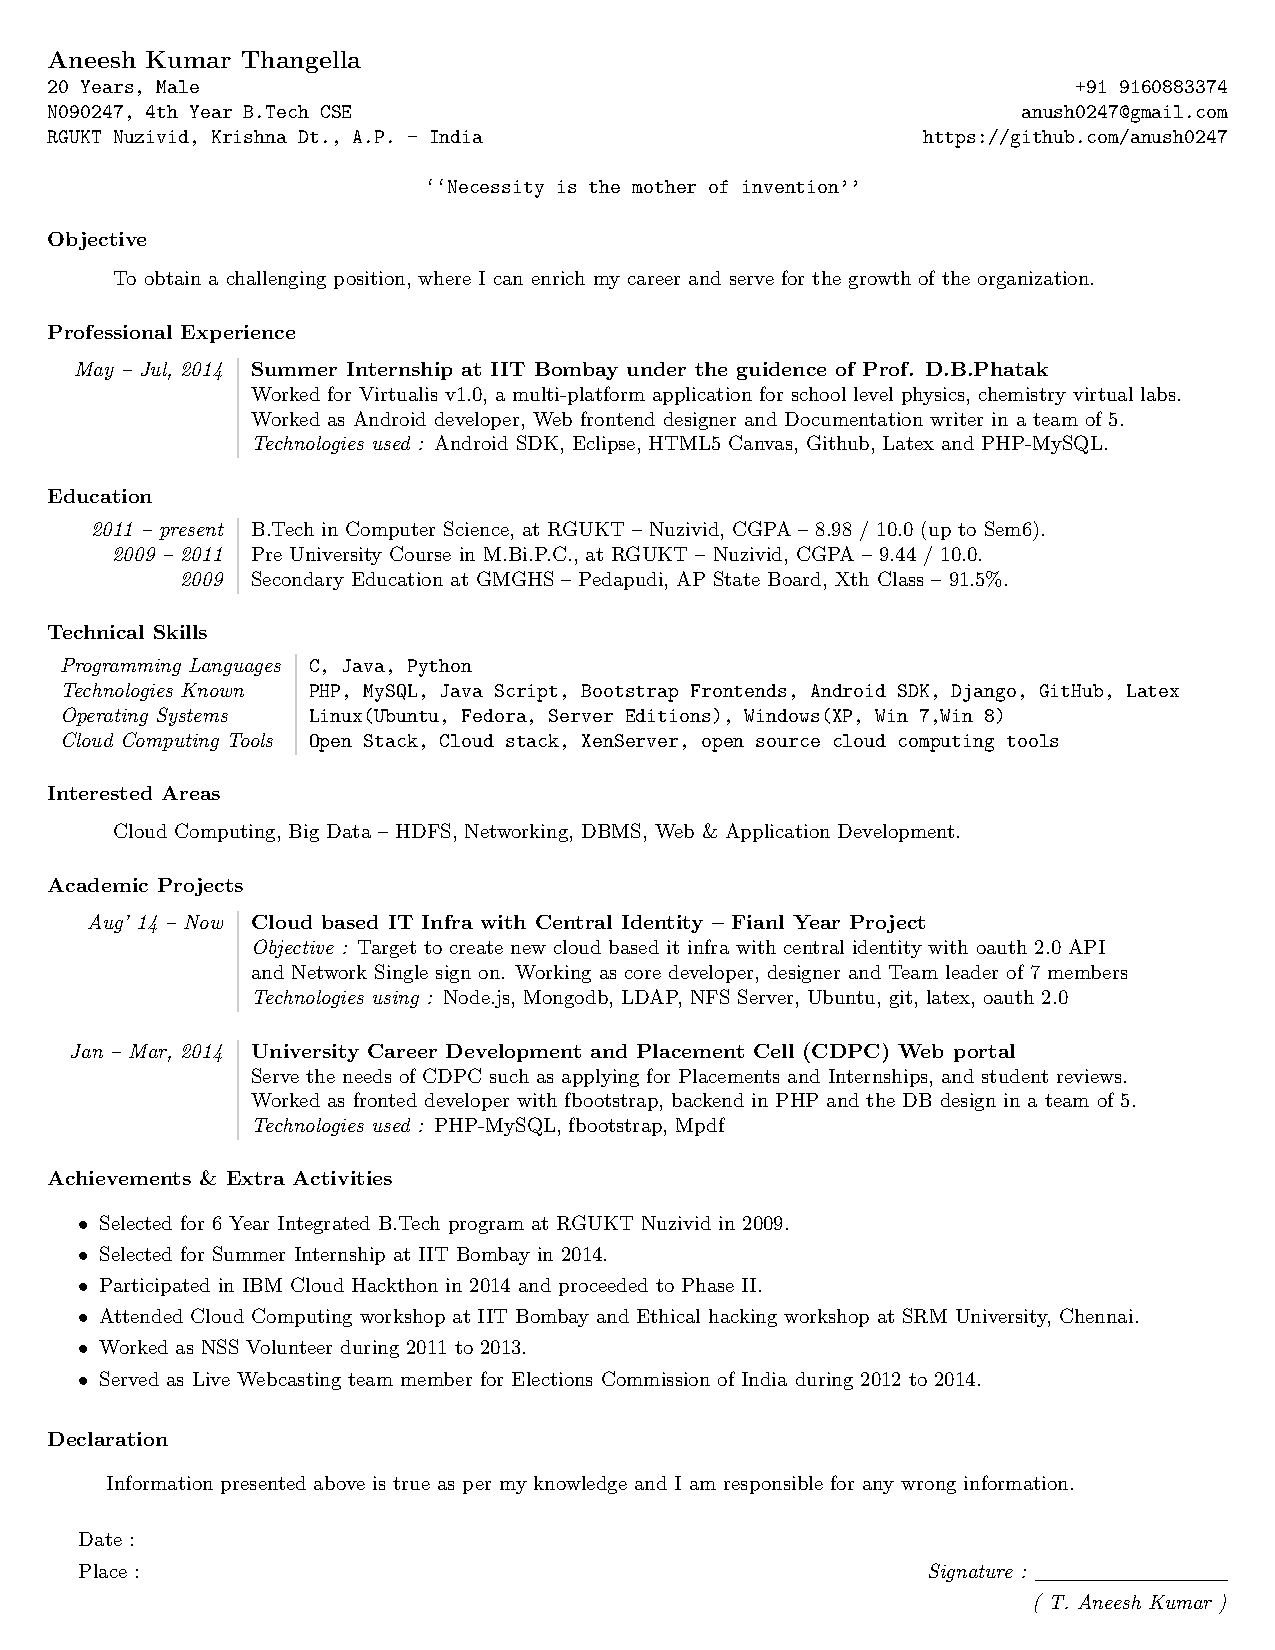
\includegraphics[width=2cm, height = 2.5cm]{aneesh.jpg}
%\end{flushright}

\end{flushright}
\end{multicols}


%\begin{center}
%\url{ ``Necessity is the mother of invention'' }
%\end{center} 

\subsubsection*{Objective}
\hspace{1cm} To obtain a challenging position, where I can enrich my career and serve for the growth of the organization.

\subsubsection*{Education}
\begin{tabular}{L!{\VRule}R}
\textit{2011 -- present} & B.Tech in Computer Science, at RGUKT -- Nuzvid, CGPA -- 8.98 / 10.0 (up to Sem6).\\
\textit{2009 -- 2011 }&  Pre University Course in M.Bi.P.C., at RGUKT -- Nuzvid, CGPA -- 9.44 / 10.0.\\
\textit{2009 } &  Secondary Education at GMGHS -- Pedapudi, AP State  Board, Xth Class -- 91.5\%.\\
\end{tabular}

\subsubsection*{Professional Experience}
\begin{tabular}{L!{\VRule}R}
\textit{ May -- Jul, 2014}&{\bf Summer Internship at IIT Bombay under the guidence of Prof. D.B.Phatak} \\
& Worked for Virtualis v1.0, a multi-platform application for school level physics, chemistry virtual labs. \\
& Worked as Android developer, Web frontend designer and Documentation writer in a team of 5. \\
& \textit{Technologies used :} Android SDK, Eclipse, HTML5 Canvas, Github, Latex and PHP-MySQL.\\
\end{tabular}

\subsubsection*{Technical Skills}
\begin{tabular}{l !{\VRule} R}
\textit{Programming Languages} &  \url{C, Java, Python }\\
\textit{Technologies Known}&	\url{PHP, MySQL, Java Script, Bootstrap Frontends, Android SDK, Django, GitHub, Latex} \\
\textit{Operating Systems} &	\url{Linux(Ubuntu, Fedora, Server Editions), Windows(XP, Win 7,Win 8) }\\
\textit{Cloud Computing Tools} 	&	\url{Open Stack, Cloud stack, XenServer, open source cloud computing tools} \\
\end{tabular}

\subsubsection*{Interested Areas of Working}
%\hspace{1cm} Cloud Computing, Big Data -- HDFS, Networking \& Databases, GUI Design, Web \& Application Development.
\onehalfspacing
\begin{compactitem}
	\item Cloud Computing, Big Data -- HDFS
	\item Networking \& Databases
	\item GUI Design \& Development
	\item Web \& Application Development
\end{compactitem}



\subsubsection*{Academic Projects}
\begin{tabular}{L!{\VRule}R}
\textit{ Aug' 14 -- Now}&{\bf Cloud based IT Infra with Central Identity -- Final Year Project } \\
& \textit{Objective :} Target to create new cloud based it infra with central identity with oauth 2.0 API\\
& and Network Single sign on. Working as core developer, designer and Team leader of 7 members \\
& \textit{Technologies using:} Node.js, Mongodb, LDAP, NFS Server, Ubuntu, git, latex, oauth 2.0\\
& \textit{Github Repo : }\url{https://github.com/reboot14/rinfra/}\\
\end{tabular}
\newline \linebreak \\
\begin{tabular}{L!{\VRule}R}
\textit{ Jan -- Mar, 2014}&{\bf University Career Development and Placement Cell (CDPC) Web portal} \\
& Serve the needs of CDPC such as applying for Placements and Internships, and student reviews.\\
& Worked as fronted developer with fbootstrap, backend in PHP and the DB design in a team of 5. \\
& \textit{Technologies used :} PHP-MySQL, fbootstrap, Mpdf\\
& \textit{Hosted at : }\url{http://rgukttnp.rgukt.in:8888/cdpc/}\\
\end{tabular}
\newline \linebreak \\
\begin{tabular}{L!{\VRule}R}
\textit{ Jun -- Aug, 2013}&{\bf Departmental Online Attendance Portal} \\
& Serve the attendance related needs like end semester eligibility and monthly reports and statistics.\\
& Worked as fronted developer with Bootstrap, backend in PHP and the DB design in a team of 5. \\
& \textit{Technologies used :} PHP-MySQL, Bootstrap, Mpdf, Flash Charts for plotting daily submissions\\
\end{tabular}

\pagebreak 

\subsubsection*{Achievements \& Postions}
%\begin{spacing}{onehalfspacing}
\onehalfspacing
\begin{compactitem}
	\item Selected for 6 years integrated B.Tech program at RGUKT Nuzvid in 2009.
	\item Selected for Summer Internship at IIT Bombay in 2014.
	\item Participated in IBM Cloud Hackthon in 2014 and qualified for phase II.
	\item Secured 1st position in CTF at TeckZite'14, Technical Fest at RGUKT - Nuzvid.
	\item Secured campus top 50th rank in Internatioanl Maths Olympiad in 2010.  
\end{compactitem}
%\end{spacing}

\subsection*{Extra Academic Activities}
\onehalfspacing
\begin{compactitem}
	\item Attended Cloud Computing workshop in TechFest'14 at IIT Bombay. 
	\item Attended Ethical hacking workshop in E-Hack'14 at SRM University, Chennai.
	\item Presentation by me on Virtualization at RGUKT, Nuzvid in Techno Start -2013.
	\item Worked as NSS volunteer during 2011 to 2013.
	\item Currently working in CSE Dept. Technical support team from 2013. 
	\item Served as Live Webcasting team member for Elections Commission of India during 2012 to 2014.
\end{compactitem}

\subsection*{Personal Assets}
\onehalfspacing
\begin{compactitem}
	\item Active team member and leader
	\item Quick Learning Ability
	\item Punctual \& Self obedient
%	\item Optimistic \& Enthusiastic
	\item Service minded \& Eco loving
\end{compactitem}

\subsection*{Personal Information}
\begin{tabular}{L!{\VRule}R}
\textit{ Father Name }&China Venkata Ramana\\
\textit{ Mother Name }&Subbayyamma\\
%\textit{ Sisters Names }& Aruna Devi, Satya Gowri\\
\textit{ Date of Birth }& 06 Feb, 1994\\
\textit{ Languages}& English (Read, Write, Speak), Telugu (Read, Write, Speak)\\
%\textit{ }& \\
\textit{Hobbies } & Listening to music, Web surfing, Playing shuttle, chess \\
%\textit{Religion } & Hindu
\end{tabular}

\subsection*{Address for Communication}
\begin{tabular}{L!{\VRule} R}
\textit{ Door No  }& 5 - 73\\
\textit{ Street Name }& New Gowri Devi Temple St.\\
\textit{ Village  }& Pedapudi \\
%\textit{ Mandal Name }& Pedapudi Mandal \\
\textit{ City \& Dist.  }& Kakinada, East Godavari Dist.\\
\textit{ State }& Andhra Pradesh\\
\textit{ Country  } & India -- 533006\\
%\textit{ Pincode }& 533006
\end{tabular}\\

\subsubsection*{Declaration}
\hspace{1cm}Information presented above is true as per my knowledge and I am responsible for any wrong information.

\begin{multicols}{2}
 Date : \\
 \indent Place : 
\begin{flushright}
\underline{} \\
\textit{
 Signature : \underline{ \hspace{3cm} } \\
  ( T. Aneesh Kumar )
}
\end{flushright}
\end{multicols}

\end{document}